%==============================
\section{Introduction}\label{sec:intro}
In many real-world scenarios, the path of a large vehicle or transport unit is obstructed by
movable obstacles such as pallets, boxes, or equipment, which motivates the use of a fleet of
mobile robots to actively clear traversable corridors and enable safe passage. This capability
is especially critical in unstructured or cluttered workspaces, including warehouses, disaster
sites, and crowded urban environments, where traditional path planning approaches assume
static obstacles and therefore fail to provide feasible solutions when direct paths are
blocked~\cite{}. Research on Navigation Among Movable Obstacles (NAMO) has proposed strategies
for pushing, pulling, or rotating objects to create new routes~\cite{}, but these methods often
abstract away physical feasibility, ignoring key factors such as robot dimensions, obstacle
size and mass, contact geometry, applied forces, and the coupled dynamics of pushing. As a
result, the generated plans may be theoretically valid but physically unrealizable in practice.
This problem is particularly challenging because a single large robot is often unable to
independently clear a corridor; smaller robots are constrained by their limited size and reach,
making some obstacle boundaries inaccessible; and pushing actions introduce strong physical
coupling, where a single push may trigger chained motions of multiple obstacles, further
complicating prediction and planning.

%==============================
\begin{figure}[t!]
  \centering
  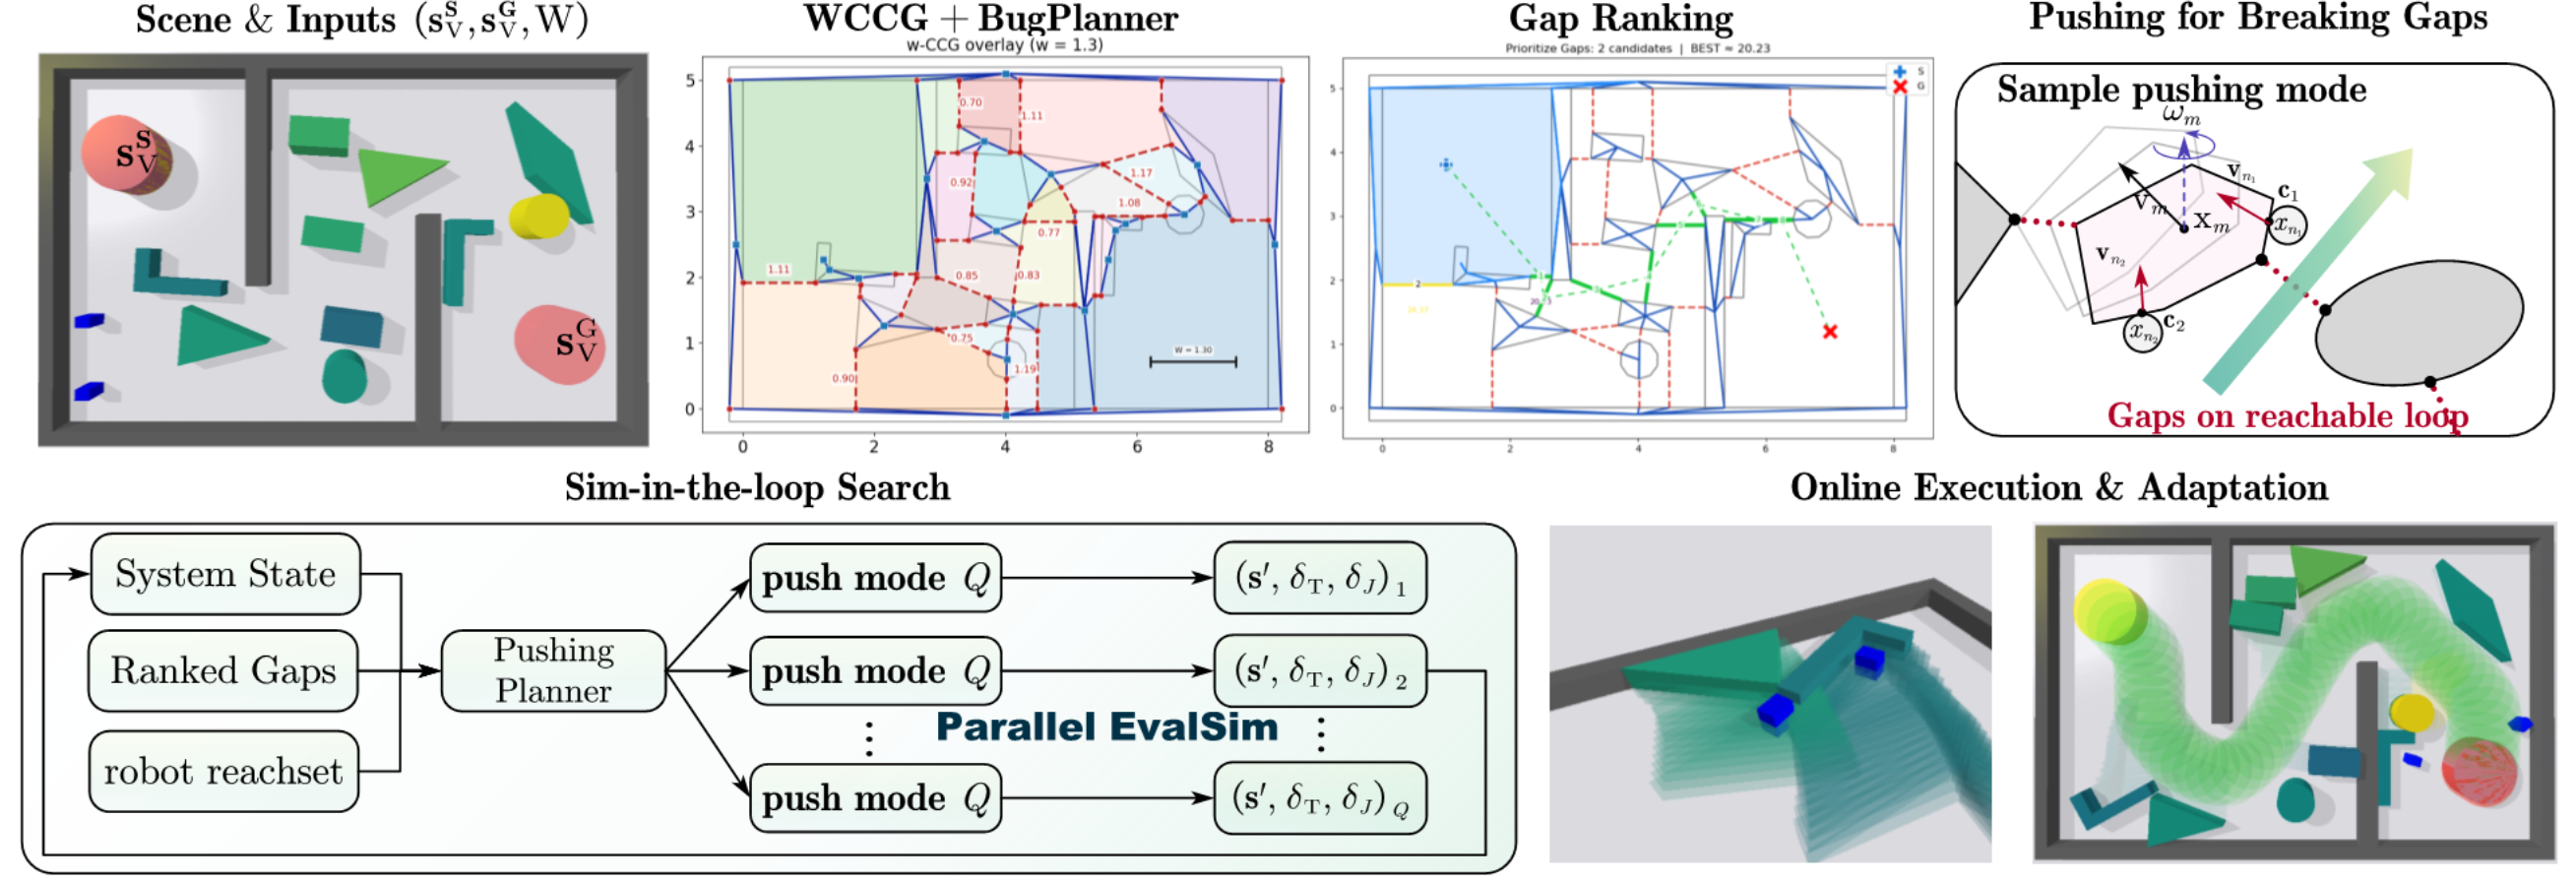
\includegraphics[width=0.95\hsize]{figures/overall.png}
  \vspace{-0.1in}
  \caption{}
  \label{fig:overall}
  \vspace{-0.2in}
\end{figure}
% ==============================

%==============================
\subsection{Related Work}\label{subsec:intro-related}

Navigation Among Movable Obstacles (NAMO) has been studied as a core
extension of motion planning in cluttered environments. Early approaches
planned sequences of obstacle displacements through pushing, pulling, or
rotating actions~\cite{}. Heuristic search methods improved scalability
by prioritizing which obstacles to move~\cite{}, and graph- or
sampling-based algorithms enabled planning in larger workspaces~\cite{}.
Multi-agent variants have also been explored~\cite{}. Despite these
advances, most NAMO approaches neglect physical feasibility, typically
treating robots as point agents with unlimited power and ignoring
dimensions, object mass, contact geometry, and force constraints. As a
result, many generated plans remain physically unrealizable~\cite{}.

Collaborative pushing has also been investigated in the context of
multi-robot manipulation. Prior work has addressed synchronization of
forces~\cite{}, stable contact maintenance~\cite{}, and cooperative
transport of objects in structured settings~\cite{}. These approaches
demonstrate effective coordination but generally focus on a single object
type and assume strict collision avoidance with surrounding obstacles.
Such assumptions exclude the possibility of exploiting inter-object
interactions, and the challenges of coupled dynamics and chain reactions
remain largely unaddressed~\cite{}.

Physics-informed planning has recently emerged to incorporate realistic
dynamics into motion planning. Some methods employ physics engines to
validate candidate manipulations~\cite{} or simulate contact dynamics
during planning~\cite{}. While these works highlight the benefits of
embedding physics, they are mostly limited to single-object manipulation
or grasp planning. In addition, many approaches decouple abstract
planning from low-level physics checks~\cite{}, which reduces efficiency,
and simulation-in-the-loop techniques face scalability challenges in
multi-robot, cluttered scenarios~\cite{}. A unified framework that
couples collaborative planning with physics-based feasibility for robust
path clearing has yet to be established.

%==============================
\subsection{Our Method}\label{subsec:intro-our}

This work introduces a physics-informed framework for collaborative multi-robot
pushing that actively constructs traversable corridors for large vehicles in
cluttered environments. The approach integrates three key components: a
W-Clearance Connectivity Graph (WCCG) to represent workspace connectivity under
vehicle width constraints and to identify blocking frontier gaps; a gap-ranking
strategy that estimates the cost of clearing each gap and prioritizes obstacles
for coordinated pushing; and a simulation-in-the-loop path construction scheme
that incrementally expands a configuration-space search tree and validates each
pushing mode through parallel physical simulation. This combination ensures that
planned actions account for robot dimensions, contact geometry, applied forces,
and chained obstacle motions, enabling physically feasible execution. The
framework is evaluated through extensive 2D and large-scale simulations as well
as hardware experiments, demonstrating robustness
under various dense obstacle configurations, and varying
team sizes.

The contributions of this work are twofold: (I) it presents the first unified
framework that couples multi-robot collaborative pushing with simulation-in-the-loop
planning to construct physically feasible paths in cluttered environments; (II)
it demonstrates significant improvements in feasibility, efficiency,
and scalability compared to existing NAMO and collaborative pushing approaches.
